%% =====================================================================
%%  MLEE Course Project Poster  (BITS Pilani, EEE Department)
%%  Built on the course template MLEE_Poster_Template.tex: same class, options, colour style,
%%  title style, blocks and block order. Guideline text and the "Poster Guidelines" block removed.
%%  Build  : pdflatex MLEE_Poster.tex (run twice)   or   tectonic MLEE_Poster.tex
%%  Figures: fig_method.pdf (report Fig. 3, draw.io), fig_background.pdf, fig_result1.pdf,
%%           fig_result2.pdf (make_poster_figs.py, drawn at printed size). Numbers match the report.
%% =====================================================================
\documentclass[30pt, a0paper, portrait, margin=0mm, innermargin=15mm,
               blockverticalspace=15mm, colspace=15mm, subcolspace=8mm]{tikzposter}

\usepackage[T1]{fontenc}
\usepackage[scaled]{helvet}
\renewcommand{\familydefault}{\sfdefault}
\usepackage{amsmath, amssymb}
\usepackage{booktabs}
\usepackage{enumitem}
\usepackage{graphicx}
\usepackage{colortbl}
\usepackage{textcomp}
\newcommand{\sci}[2]{#1\,$\times$\,10\textsuperscript{\textminus#2}}   % 5.0 x 10^-7 in the text font

% ---------------------------------------------------------------------
%  FILE NAMES
% ---------------------------------------------------------------------
\newcommand{\bitslogofile}{bits_logo.png}      % BITS Pilani logo

% ---------------------------------------------------------------------
%  COLOURS  (BITS-style navy and blue, as in the template)
% ---------------------------------------------------------------------
\definecolor{bitsnavy}{HTML}{1F3864}
\definecolor{bitsblue}{HTML}{2E75B6}
\definecolor{bitsgold}{HTML}{C9A227}
\definecolor{guidegrey}{HTML}{5F5F5F}
\definecolor{ourgreen}{HTML}{2E8B57}
\definecolor{paleblue}{HTML}{EAF1FB}

\definecolorstyle{BITSStyle}{
  \colorlet{colorOne}{bitsnavy}
  \colorlet{colorTwo}{bitsblue}
  \colorlet{colorThree}{bitsgold}
}{
  \colorlet{backgroundcolor}{white}
  \colorlet{framecolor}{bitsnavy}
  \colorlet{titlefgcolor}{white}
  \colorlet{titlebgcolor}{bitsnavy}
  \colorlet{blocktitlebgcolor}{bitsblue}
  \colorlet{blocktitlefgcolor}{white}
  \colorlet{blockbodybgcolor}{white}
  \colorlet{blockbodyfgcolor}{black}
  \colorlet{innerblocktitlebgcolor}{bitsblue}
  \colorlet{innerblocktitlefgcolor}{white}
  \colorlet{innerblockbodybgcolor}{white}
  \colorlet{innerblockbodyfgcolor}{black}
  \colorlet{notefgcolor}{black}
  \colorlet{notebgcolor}{bitsblue!10}
  \colorlet{noteframecolor}{bitsblue}
}
\usecolorstyle{BITSStyle}
\usetitlestyle[width=0.97\textwidth]{Default}
\useblockstyle{Default}
\usebackgroundstyle{Default}

% ---------------------------------------------------------------------
%  HELPER MACROS (template)
% ---------------------------------------------------------------------
\newcommand{\logoslot}[1]{\includegraphics[height=7cm, width=\linewidth, keepaspectratio]{#1}}
\newcommand{\fig}[2]{\begin{center}\includegraphics[width=#2]{#1}\end{center}\vspace{-6mm}}
\newcommand{\figcap}[1]{{\par\centering\small\itshape #1\par}\vspace{4mm}}
\setlist[itemize]{leftmargin=1.2em, itemsep=6pt, topsep=4pt, parsep=0pt, before=\raggedright}
\setlist[enumerate]{leftmargin=1.5em, itemsep=6pt, topsep=4pt, parsep=0pt, before=\raggedright}
\hyphenpenalty=10000 \exhyphenpenalty=10000   % no hyphenation on a poster

% Headline number for the summary block: #1 colour, #2 number, #3 label
\newcommand{\kpi}[3]{%
  \begin{tikzpicture}
    \node[fill=paleblue, draw=#1, line width=3pt, rounded corners=12pt, minimum width=0.23\linewidth,
          minimum height=7.8cm, inner sep=0pt] (b) {};
    \node[anchor=north, text=#1, font=\bfseries\fontsize{60}{66}\selectfont] at ([yshift=-0.7cm]b.north) {#2};
    \node[anchor=north, text width=0.2\linewidth, align=center, font=\fontsize{25}{30}\selectfont]
         at ([yshift=-3.5cm]b.north) {#3};
  \end{tikzpicture}}

% ---------------------------------------------------------------------
%  TITLE, TEAM, AFFILIATION
% ---------------------------------------------------------------------
\title{Low-Complexity Neural Network Equalization for Optical Fibre Communication on FPGA}
% tikzposter measures \@title in an unbreakable box, so the two-line title is set directly in \settitle below
\newcommand{\posterTitle}{Low-Complexity Neural Network Equalization\\for Optical Fibre Communication on FPGA}
\author{[Student Name 1] \;\textbullet\; [Student Name 2] \;\textbullet\; [Student Name 3]
        \;\;|\;\; Team [ID]}
\institute{Department of Electrical and Electronics Engineering, BITS Pilani, Pilani Campus
           \;\textbullet\; MLEE \;\textbullet\; Instructor: Dr. Ritesh Vyas \;\textbullet\; Semester I, 2026--27}

\makeatletter
\settitle{%
  \centering
  \begin{minipage}[c]{0.16\linewidth}\centering
    \logoslot{\bitslogofile}
  \end{minipage}%
  \begin{minipage}[c]{0.64\linewidth}\centering\color{titlefgcolor}
    {\bfseries\fontsize{64}{72}\selectfont \posterTitle \par}
    \vspace{1.2em}
    {\fontsize{36}{44}\selectfont \@author \par}
    \vspace{0.6em}
    {\fontsize{28}{34}\selectfont \@institute \par}
  \end{minipage}%
}
\makeatother

\begin{document}
\maketitle

% =====================================================================
\begin{columns}
% ------------------------- LEFT COLUMN -------------------------------
\column{0.5}

\block{Summary}{
  We rebuilt the CNN equalizer of Ney et al.\ [8] for a 40\,GBd, 31.5\,km optical link and improved it with a
  \textbf{decision-aligned loss}, \textbf{decision feedback} and a \textbf{hand-written FPGA engine}.
  \vspace{4mm}

  \noindent\kpi{bitsblue}{16$\times$}{lower BER, same complexity budget}\hfill
  \kpi{ourgreen}{$\approx$1000$\times$}{lower BER at 8 bits, with feedback}\hfill
  \kpi{bitsnavy}{200\,MHz}{in the full PYNQ-Z2 system}\hfill
  \kpi{bitsnavy}{$-$23\,\%}{LUTs vs the paper's CNN, same engine}
}

\block{Introduction and Objectives}{
  \textbf{Motivation:} cheap IM/DD links turn fibre dispersion into spectral nulls that linear equalizers cannot
  fill; neural equalizers help, but must run in real time.
  \vspace{2mm}

  \textbf{Objectives:}
  \begin{itemize}
    \item Reproduce the paper's CNN from scratch: simulator and strong baselines.
    \item Improve accuracy at equal cost: loss, topology, decision feedback.
    \item Deploy bit-exact integer models at 200\,MHz on a PYNQ-Z2.
  \end{itemize}
}

\block{Background}{
  \begin{minipage}[c]{0.6\linewidth}
    \textbf{Key idea:} dispersion + square-law detection $\to$ \emph{power fading} [3]:
    \[ |H(f)| = \left|\cos\!\left(2\pi^2 \beta_2 L f^2\right)\right| \]
    \vspace{-8mm}
    \begin{itemize}
      \item Paper [8]: CNN + HLS design, MSE loss, FIR baseline only.
      \item Decision feedback: textbook fix for nulls [9].
      \item \textbf{Gap:} aligned loss, feedback baselines, real power.
    \end{itemize}
  \end{minipage}\hfill
  \begin{minipage}[c]{0.38\linewidth}
    \centering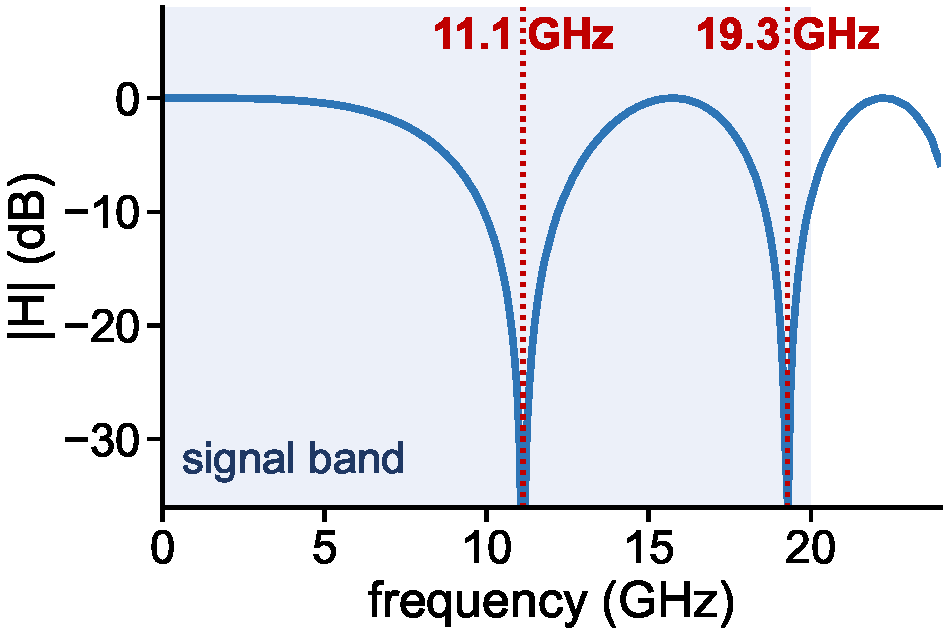
\includegraphics[width=\linewidth]{fig_background.pdf}
  \end{minipage}
}

\block{Methodology}{
  \fig{fig_method.pdf}{0.86\linewidth}
  \figcap{Figure 1: (a) PYNQ-Z2 system: DMA at 100\,MHz, equalizer at 200\,MHz. (b) Each convolution layer is a pipeline that never stalls internally.}
  \begin{enumerate}
    \item \textbf{Data:} physical IM/DD simulator; 2M train, 2M select, fresh 4M test.
    \item \textbf{Models:} 135 CNN topologies $\times$ 2 losses; FIR, Volterra, FFE+DFE, MLSE.
    \item \textbf{Quantization:} QAT [16] to 3--8 bit; integer golden model = exact RTL.
    \item \textbf{Hardware:} shared multipliers, 2 channels / DSP, look-ahead DFE.
  \end{enumerate}
}

\block{Experimental Setup}{
  {\centering
  \begin{tabular}{ll}
    \toprule
    \textbf{Parameter} & \textbf{Value / description} \\
    \midrule
    Link          & 40\,GBd PAM2, 31.5\,km SSMF, 2 samples / symbol, 24\,dB SNR \\
    CNN training  & Adam, rate 10\textsuperscript{\textminus3}, 10k iterations, 3 seeds; MSE vs cross-entropy \\
    Quantization  & QAT, weights = activations = input = 3--8 bit \\
    Hardware      & XC7Z020-1 (PYNQ-Z2), Vivado 2025.2; power from SAIF \\
    \bottomrule
  \end{tabular}\par}
}

% ------------------------- RIGHT COLUMN ------------------------------
\column{0.5}

\block{Results}{
  \fig{fig_result1.pdf}{0.97\linewidth}
  \figcap{Figure 2: The same budget buys 16$\times$ lower BER with cross-entropy and a 4-layer CNN. As deployed
  integers, two feedback taps reach \sci{5.0}{7} (2 errors in 4M bits).}

  \begin{center}
  \setlength{\tabcolsep}{9pt}
  \begin{tabular}{lcccccc}
    \toprule
    \textbf{Design} (DSP build) & \textbf{BER} & \textbf{MHz} & \textbf{LUT} & \textbf{FF} & \textbf{DSP} & \textbf{Power} \\
    \midrule
    Paper's CNN, 8 bit     & \sci{4.96}{4} & 187.9 & 7,056 & 11,543 & 42 & 0.302\,W \\
    Ours, CNN, 6 bit       & \sci{2.18}{5} & 207.2 & 3,957 & 6,393  & 45 & 0.259\,W \\
    \rowcolor{paleblue}
    \textbf{Ours, CNN + DFE, 8 bit} & \textbf{\sci{5.0}{7}} & \textbf{202.4} & \textbf{5,430} & \textbf{8,919}
                                     & \textbf{43} & \textbf{0.318\,W} \\
    \bottomrule
  \end{tabular}
  \end{center}
  \figcap{Table 1: Same engine, same XC7Z020: 23--44\,\% fewer LUTs. Dynamic power at 200\,MHz from simulated activity.
  All six routed builds are bit-exact at gate level.}

  \fig{fig_result2.pdf}{0.97\linewidth}
  \figcap{Figure 3: BER over nine channel conditions (best per row outlined; multiplications per symbol in brackets).
  At 31.5\,km and $\ge$\,16\,dB a 59-multiplication FFE + DFE wins; the CNN + DFE wins on the hardest channels.}
}

\block{Discussion}{
  \begin{itemize}
    \item \textbf{Finding:} decision feedback, absent from the paper, is the strongest single idea: it fills the
          fading nulls that no feed-forward equalizer can.
    \item \textbf{Finding:} the loss and the topology work together: the 4-layer CNN fails with MSE and is the best
          with cross-entropy.
    \item \textbf{Limitation:} at 24\,dB a 27-multiplication FFE + DFE matches our \sci{5.0}{7}; the CNN's
          case is robustness on harder channels. All data are simulated, and \sci{5.0}{7} rests on 2 errors
          (still $\ge$\,270$\times$ better at 95\,\% confidence).
  \end{itemize}
}

\block{Conclusion and Future Work}{
  \begin{itemize}
    \item At the same 8 bits, our CNN + DFE has about 1000$\times$ lower BER than the paper's CNN and runs at
          200\,MHz on a PYNQ-Z2 with 23\,\% fewer LUTs.
    \item The paper's multiplication count is low by a factor of 2; multiplier sharing and two channels per DSP cut 136 to 45 DSPs.
    \item \textbf{Future work:} measure BER and power on the board, train on the lab's fibre kit, a parallel
          look-ahead DFE towards 40\,GBd, and a LUT-native KAN equalizer [15].
  \end{itemize}
}

\begin{subcolumns}
\subcolumn{0.62}
\block{References}{
  {\small
  \begin{enumerate}[leftmargin=2.2em, itemsep=3pt]
    \item[{[3]}] G.~J. Meslener, ``Chromatic dispersion induced distortion of modulated monochromatic light employing
          direct detection,'' \emph{IEEE J. Quantum Electron.}, vol.~20, no.~10, pp.~1208--1216, 1984.
    \item[{[8]}] J. Ney \emph{et al.}, ``CNN-based equalization for communications: Achieving gigabit throughput with
          a flexible FPGA hardware architecture,'' arXiv:2405.02323, 2024.
    \item[{[9]}] J.~G. Proakis and M. Salehi, \emph{Digital Communications}, 5th ed., McGraw-Hill, 2008.
    \item[{[15]}] R. Fischer \emph{et al.}, ``Non-linear equalization in 112 Gb/s PONs using Kolmogorov-Arnold
          networks,'' in \emph{Proc.\ OFC}, 2025.
    \item[{[16]}] S.~K. Esser \emph{et al.}, ``Learned step size quantization,'' in \emph{Proc.\ ICLR}, 2020.
  \end{enumerate}}
}
\subcolumn{0.38}
\block{Report and Code}{
  {\small\raggedright
  \textbf{Report:} MLEE\_Report.pdf (numbers and reference numbers match this poster)\par\vspace{3mm}
  \textbf{Code:} github.com/JSpectre20/ mlee-cnn-equalizer (private; access on request)\par\vspace{3mm}
  \textbf{Contact:} [email]\par\vspace{3mm}
  \textbf{Thanks:} Dr. Ritesh Vyas}
}
\end{subcolumns}

\end{columns}
\end{document}
